\documentclass[10pt,journal]{IEEEtran}
\usepackage{graphicx,booktabs,multirow,amsmath,amssymb,url,xcolor}
\usepackage[caption=false,font=footnotesize]{subfig}
\graphicspath{{figures/}}
\newcommand{\mf}{macro-F1}
\title{When Shared Hyperparameters Reverse Model Rankings:\\A Controlled Study of Visual Water-Condition Classification}
\author{Anonymous Authors}
\begin{document}
\maketitle
\begin{abstract}
Comparisons between a custom architecture and pretrained baselines often reuse one training configuration for every model. We show that this apparently controlled choice can systematically favor the custom model. Using seven-class visual water-condition classification as a case study, we evaluate ten architectures with an identical tuning budget, five promotion seeds, and per-image predictions. The best-to-worst validation \mf{} spread within the same six-setting grid ranges from 0.032 for the proposed AquaNet to 0.190 for ResNet-50. Under the shared setting AquaNet appears strongest; after model-wise validation selection it ranks ninth of ten, is below a statistically indistinguishable top group, and is worse than its unmodified DenseNet-121 backbone. A 69-run factorial ablation and parameter-matched neck control show that its two proposed modules are null-to-negative. The conclusion persists across calibration, abstention, corruptions and a 146-image out-of-distribution set. These results turn an apparent architecture gain into a quantified evaluation-protocol effect and motivate equal tuning budgets, rather than equal hyperparameter values, as the appropriate control.
\end{abstract}
\begin{IEEEkeywords}benchmarking, hyperparameter tuning, pretrained models, water-condition recognition, reproducibility, negative results
\end{IEEEkeywords}

\section{Introduction}
Vision models are increasingly used to screen waterways from cameras and drones, complementing but not replacing physical sensing \cite{al2024drone,kim2023cctv}. At the same time, architectural papers commonly compare a proposed network containing freshly initialized layers with ImageNet-pretrained baselines. Giving every model the same learning rate looks fair, yet it equalizes a value rather than the opportunity to find an appropriate value. The proposed and baseline models may occupy very different optimization regimes.

This study began as an attempt to validate AquaNet, a DenseNet-based network augmented with a multi-scale residual block (MSRB), channel-spatial attention block (CSAB), and optional hierarchical head. The initial shared-hyperparameter experiments suggested that it beat common baselines. A diagnostic tuning grid reversed that result. This reversal is the main finding rather than an inconvenience to hide.

Our contributions are: (1) a controlled measurement of model-dependent hyperparameter sensitivity across ten CNN and transformer configurations; (2) a five-seed comparison using equal tuning budgets, paired tests and Holm correction; (3) a full head$\times$MSRB$\times$CSAB factorial with a parameter-matched control, establishing a well-supported negative architecture result; and (4) evaluation on calibration, selective prediction, corruptions, out-of-distribution (OOD) transfer and explanation faithfulness. We make no claim that RGB appearance measures physicochemical water quality: the task is seven-class \emph{surface-condition recognition}.

\section{Related Work}
Our model set spans ResNet \cite{he2016resnet}, DenseNet \cite{huang2017densenet}, MobileNetV2 \cite{sandler2018mobilenet}, EfficientNet \cite{tan2019efficientnet}, ConvNeXt \cite{liu2022convnext}, DeiT \cite{touvron2021deit}, and Swin Transformer \cite{liu2021swin}. AquaNet uses attention related to CBAM \cite{woo2018cbam}. Calibration and gradient localization follow temperature scaling \cite{guo2017calibration} and Grad-CAM \cite{selvaraju2017gradcam}.

Our methodological concern is related to evidence that benchmark rankings vary with seeds and experimental budgets \cite{bouthillier2021variance,lucic2018gans}. We isolate a specific asymmetry: a shared learning rate can advantage a custom head/neck with millions of new parameters over a nearly fully pretrained baseline. The relevant fairness unit is therefore the \emph{search budget and selection rule}, not a common scalar value.

\section{Data and Task}
The primary set D1 contains 2,799 images in seven labels: clean, algae, debris, foam, oil, turbid, and uncertain. The fixed train/validation/test split contains 1,956/416/427 images. D2 contains 213 real-video frames for adaptation and D3 contains 146 held-out web/video images for OOD testing. Exact MD5 duplicates were removed before splitting; a perceptual-hash audit retained 698 candidate pairs for manual sensitivity analysis. D1 originated from a public Kaggle collection and includes generated images, so it is neither introduced nor named here as a novel dataset. This provenance limits ecological conclusions.

Let $f_\theta(x)$ output probabilities $p\in\mathbb{R}^7$. The primary metric is class-balanced
\begin{equation}
 \mathrm{mF1}=\frac{1}{7}\sum_{c=1}^{7}\frac{2P_cR_c}{P_c+R_c}.
\end{equation}
Weighted cross entropy, $\mathcal{L}=-\sum_c w_c y_c\log p_c$, is used for all models. Validation \mf{}, never test performance, selects checkpoints and hyperparameters.

\section{Models and Controlled Protocol}
\subsection{AquaNet case-study architecture}
The model combines a pretrained DenseNet-121 trunk with an MSRB, CSAB and either a flat softmax or a hierarchical clean/contaminated plus type head. The full flat model has 10.53M parameters; the unmodified DenseNet baseline has 6.96M. A MatchedNeck control has the same normalization count and 3.41M parameters as MSRB. Variants are denoted full (flat/on/on), no-neck (flat/off/off), and hier (hierarchical teacher forcing/on/off).

\subsection{Fairness protocol}
All inputs, splits, augmentation, loss, class balancing, epoch budget and validation rule are identical. Stage T gives each model the same six trials:
\begin{equation}
\eta\in\{10^{-4},3\!\times\!10^{-4},10^{-3}\},\quad m_b\in\{0.1,1.0\},
\end{equation}
where $m_b$ multiplies the backbone learning rate. Each model's validation-selected pair is then promoted to seeds $\{7,21,42,1337,2024\}$. This separates equal \emph{budget} from equal \emph{values}. In total, Phase 4 contains 222 successful training runs and all headline runs save per-image predictions.

For model $j$, protocol sensitivity is
\begin{equation}
 S_j=\max_{h\in\mathcal{H}}\mathrm{mF1}_{val}(j,h)-\min_{h\in\mathcal{H}}\mathrm{mF1}_{val}(j,h).
\end{equation}
Seed-matched tests use paired differences; family-wise error is controlled by Holm's procedure. We report means, sample standard deviations and 95\% $t$ intervals for five seeds.

\section{Results}
\subsection{The shared setting is not neutral}
Figure~\ref{fig:sensitivity} is the central result. Sensitivity ranges from 0.0324 for AquaNet-full to 0.1901 for ResNet-50. The three AquaNet variants are the least sensitive; several pretrained baselines are the most sensitive. Moving from the original shared setting to model-wise tuning increases test \mf{} by 0.0574 for ResNet-50, 0.0356 for EfficientNet-B0, and only 0.0101 for AquaNet. Thus a value suitable for a model with a large new neck is not a neutral setting for a nearly fully pretrained network.
\begin{figure}[t]\centering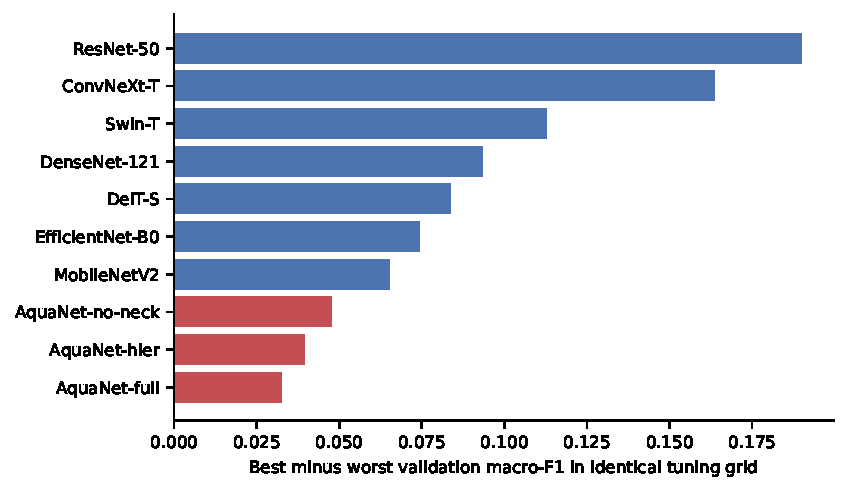
\includegraphics[width=\columnwidth]{protocol_sensitivity.pdf}\caption{Best-to-worst validation \mf{} spread within the identical six-trial budget. Red bars are AquaNet variants.}\label{fig:sensitivity}\end{figure}

\subsection{Five-seed ranking after model-wise selection}
\begin{table}[t]\centering\caption{Tuned Stage-P results (five seeds).}\label{tab:main}\scriptsize
\begin{tabular}{lrrrr}\toprule Model&Test \mf{}&SD&Acc.&Params M\\\midrule
Swin-T&\textbf{.9053}&.0094&.9283&27.52\\
DeiT-S&.8871&.0077&.9162&21.67\\ConvNeXt-T&.8851&.0102&.9162&27.83\\
ResNet-50&.8798&.0152&.9087&23.52\\DenseNet-121&.8751&.0140&.9063&6.96\\
AquaNet-hier&.8716&.0127&.9040&10.50\\AquaNet-no-neck&.8701&.0069&.9030&7.61\\
EfficientNet-B0&.8668&.0072&.8965&4.02\\AquaNet-full&.8661&.0165&.8979&10.53\\
MobileNetV2&.8425&.0205&.8815&2.23\\\bottomrule\end{tabular}\end{table}

Table~\ref{tab:main} and Fig.~\ref{fig:ranking} reverse the initial narrative. The published AquaNet configuration ranks ninth and underperforms its own DenseNet backbone despite 3.57M more parameters. Swin-T is validation-selected, but its margins over DeiT-S, ConvNeXt-T, ResNet-50 and DenseNet-121 do not survive Holm correction ($p_{Holm}=0.303,0.303,0.303,0.175$). These models form an indistinguishable top group. Swin-T does significantly exceed AquaNet-full (difference .0392, 5/5 seeds, $p_{Holm}=.0085$) and AquaNet-no-neck (.0352, 5/5, $p_{Holm}=.0199$). We therefore do not claim a universal winner.
\begin{figure}[t]\centering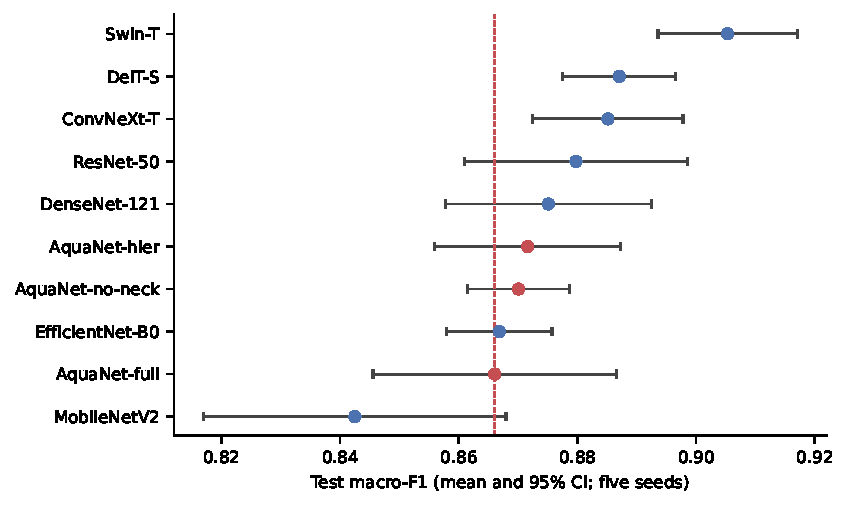
\includegraphics[width=\columnwidth]{ranking.pdf}\caption{Tuned test \mf{} with 95\% intervals. The dashed line marks AquaNet-full.}\label{fig:ranking}\end{figure}

\subsection{Factorial ablation: modules do not help}
The 69-run factorial marginal means are: head flat .8585, hier-TF .8542, hier-naive .8540; MSRB off .8604, matched .8537, on .8528; CSAB off .8586, on .8527. Across 18 matched triplets MSRB versus MatchedNeck is +.0014 with 8/18 wins, while MSRB versus no neck is $-.0053$ with 7/18 wins. The definitive tuned five-seed comparison, full versus no-neck, is $-.0040$ with 2/5 wins ($p=.61$). The modules are null-to-negative, not novel gains.

\subsection{Decision quality and robustness}
Swin-T obtains AURC .0104, accuracy at 90\% coverage .9578, binary AUROC .9922 and temperature-scaled ECE .0301. AquaNet-full obtains .0178, .9333, .9769 and .0374. DeiT-S has the lowest false-clean rate (.0135) and corruption degradation (.0255). Full and hierarchical AquaNet degrade by .0811 and .0843; removing the neck reduces this to .0479. Figure~\ref{fig:decision} summarizes the selected axes.
\begin{figure}[t]\centering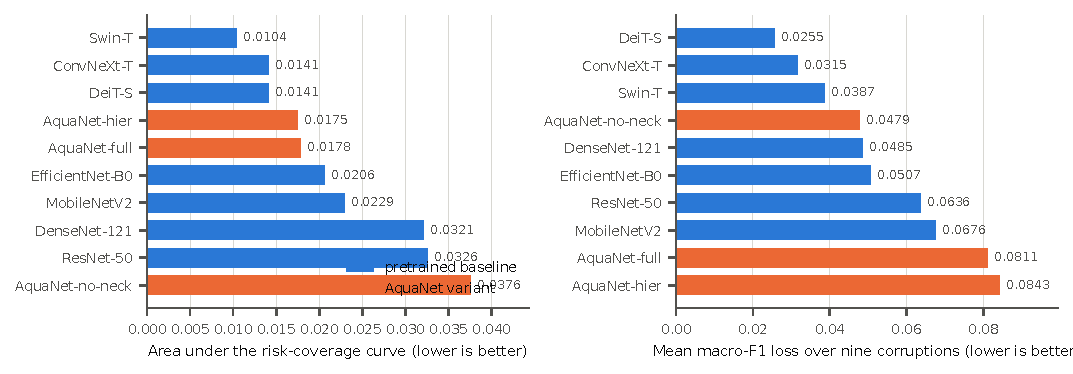
\includegraphics[width=\columnwidth]{decision_quality.pdf}\caption{Selective-prediction risk and mean corruption degradation.}\label{fig:decision}\end{figure}

\subsection{OOD transfer}
On D3, Swin-T reaches .5035 mean zero-shot \mf{}, followed by DeiT-S (.4980) and ConvNeXt-T (.4955). AquaNet-no-neck obtains .4787, whereas AquaNet-full obtains .3957. The neck penalty grows from .004 in-distribution to .083 OOD. Adaptation with 25/50/75/100\% of D2 gives .5961/.6653/.6456/.7069 mean D3 \mf{} over three seeds. The non-monotonic 75\% point and small D3 classes require caution.
\begin{figure}[t]\centering
\subfloat[Zero-shot ranking.]{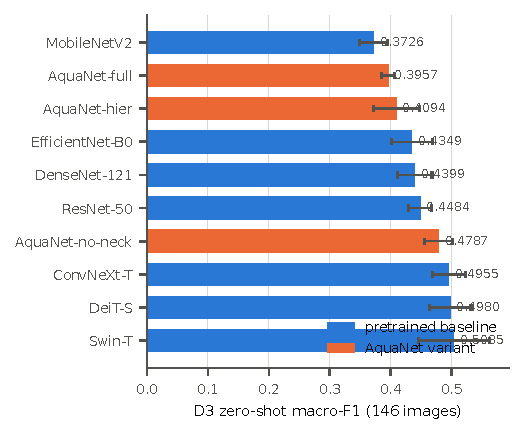
\includegraphics[width=.50\columnwidth]{ood_transfer.pdf}}
\subfloat[D2 adaptation.]{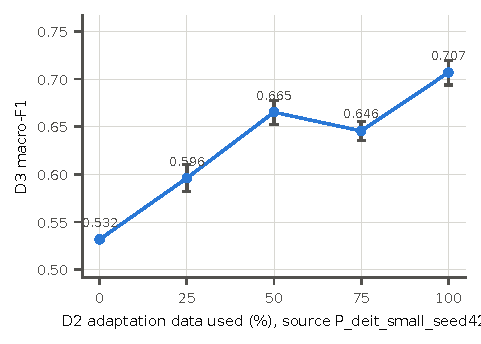
\includegraphics[width=.47\columnwidth]{adaptation.pdf}}
\caption{OOD evaluation on D3 (146 images).}\label{fig:ood}\end{figure}

\subsection{Explanation faithfulness}
Deletion/insertion evaluates whether ranked Grad-CAM pixels affect the predicted score. AquaNet-hier gives deletion/insertion AUC .7739/.9044 (gap .1305), ResNet-50 .7747/.8914, and AquaNet-no-neck .7934/.9004. AquaNet-full's gap is substantially smaller. Because gradient maps are not architecture-neutral and standard Grad-CAM is poorly matched to transformer token mixing, we treat these as within-family diagnostics, not proof that one architecture is more interpretable.
\begin{figure}[t]\centering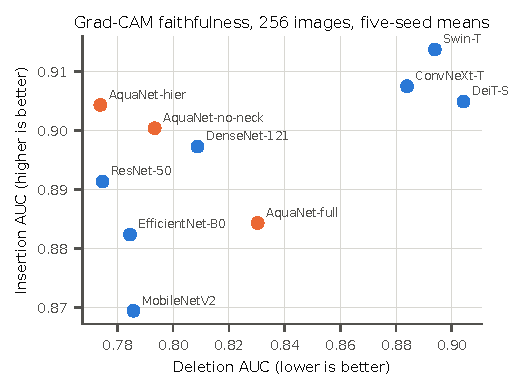
\includegraphics[width=.8\columnwidth]{explanations.pdf}\caption{Deletion--insertion operating points; upper-left is preferable.}\label{fig:explain}\end{figure}
\begin{figure}[t]\centering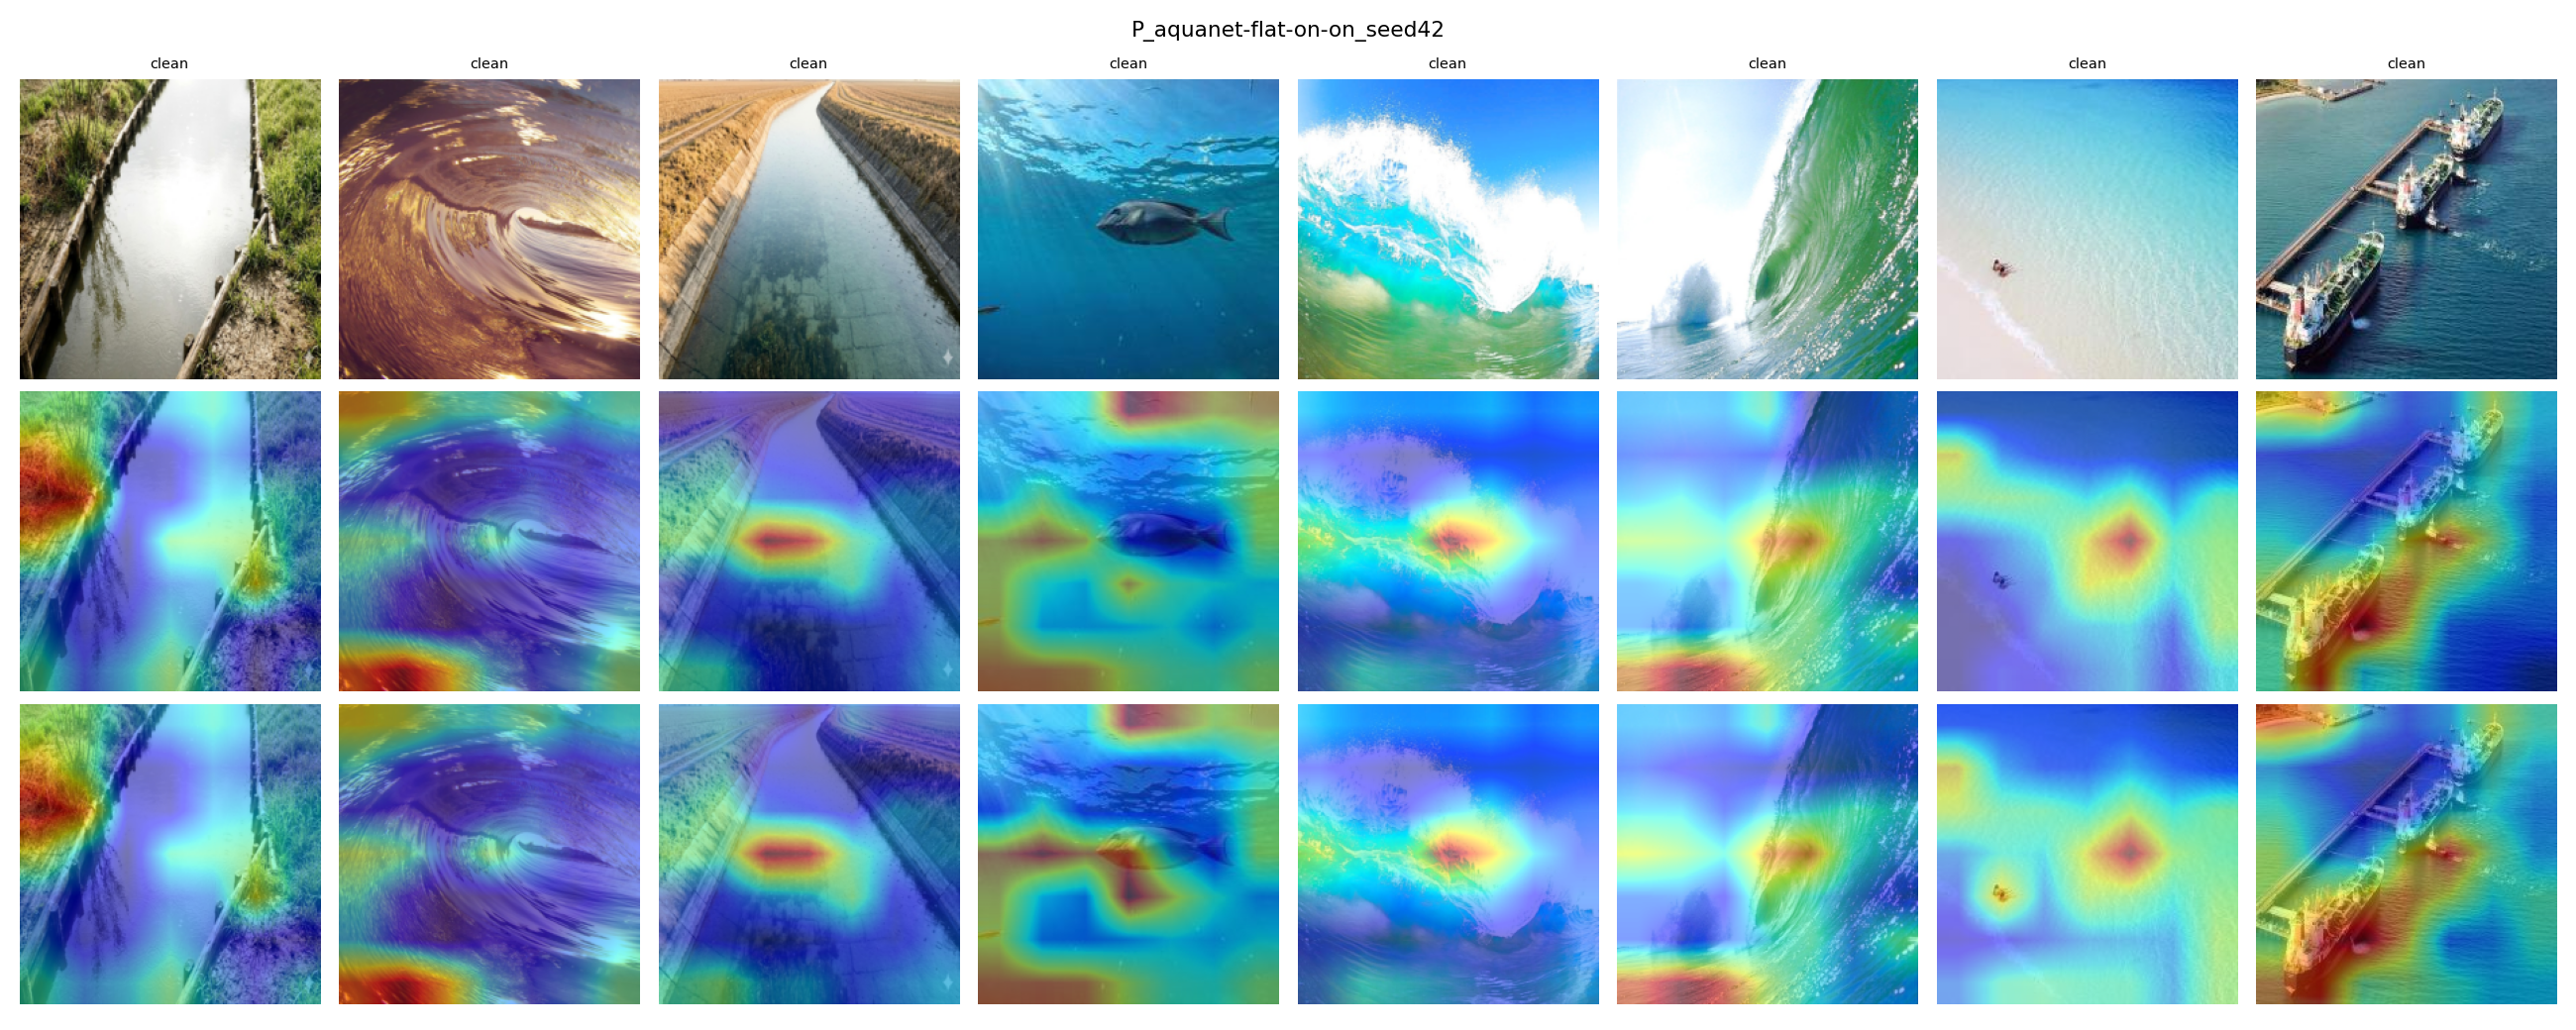
\includegraphics[width=\columnwidth]{gradcam_aquanet_seed42.png}\caption{Representative AquaNet-full Grad-CAM panel at seed 42. Qualitative maps are illustrative; quantitative deletion/insertion provides the faithfulness test.}\label{fig:gradcam}\end{figure}

\section{Discussion}
The ranking reversal has a simple mechanism. A nearly fully pretrained backbone can require conservative updates, while AquaNet includes roughly 3.5M new parameters that need larger updates. A single shared learning rate is consequently a model-specific choice disguised as a control. Equal search spaces and validation rules expose this asymmetry; they do not guarantee the globally optimal model, but they remove the observed one-sided advantage.

The result also illustrates why ablations need parameter-matched controls. Removing MSRB changes both computation and capacity; MatchedNeck isolates capacity and still finds no gain. Moreover, the architecture's weaker corruption and OOD behavior contradicts the intended generalization rationale. Negative results are valuable when they retire unsupported complexity.

Practical guidance follows. Report the search space and per-model selected values; give every model the same number of validation trials; keep test data outside selection; promote with multiple seeds; save per-example outputs; correct multiplicity; and distinguish rankings from significant groups. For deployment on this data, the evidence supports selecting within the top group using latency and resource constraints, not choosing AquaNet for architectural novelty.

\section{Limitations and Ethics}
D1 is modest, public, and partly generated; D3 contains only 146 images. Labels describe visible surface conditions, not chemical safety, and predictions must not be used as drinking-water or regulatory determinations. The six-point grid measures local sensitivity rather than exhaustive optimization. Only one task is studied, so the ranking-reversal mechanism should be tested elsewhere. Candidate perceptual duplicates and source artifacts remain possible confounders despite exact deduplication. Data and code release is planned after acceptance or on reviewer request, subject to original licenses; the experiment manifests and per-image outputs permit audit.

\section{Conclusion}
An apparent AquaNet advantage disappears under equal per-model tuning budgets. Shared hyperparameter values penalize pretrained baselines far more than the custom network, reversing the ranking. Fair tuning places AquaNet below a top group and shows that its added modules do not help. The general lesson is precise: controlled comparisons should equalize tuning opportunity, not force unlike models to share an optimization setting.

\bibliographystyle{IEEEtran}
\bibliography{references}
\end{document}
